\documentclass[honours,12pt,twoside]{unswthesis}

\usepackage{afterpage}
\usepackage{amsfonts}
\usepackage{amsmath}
\usepackage{amssymb}
\usepackage{amsthm}
\usepackage[english]{babel}
\usepackage{graphicx}
\usepackage{natbib}
\usepackage[utf8]{inputenc}
\usepackage{latexsym}
\usepackage{url}
\usepackage{todonotes}
\usepackage{tikz}
\usepackage{pdfpages}
\usetikzlibrary{arrows}
\usepackage{float}

\usepackage{booktabs}
\renewcommand{\arraystretch}{1.2}


%%%%%%%%%%%%%%%%%%%%%%%%%%%%%%%%%%%%%%%%%%%%%%%%%%%%%%%%%%%%%%%%%
%
%  The following are some simple LaTeX macros to give some
%  commonly used letters in funny fonts. You may need more or less of
%  these
%
\newcommand{\R}{\mathbb{R}}
\newcommand{\Q}{\mathbb{Q}}
\newcommand{\C}{\mathbb{C}}
\newcommand{\N}{\mathbb{N}}
\newcommand{\F}{\mathbb{F}}
\newcommand{\PP}{\mathbb{P}}
\newcommand{\T}{\mathbb{T}}
\newcommand{\Z}{\mathbb{Z}}
\newcommand{\B}{\mathfrak{B}}
\newcommand{\BB}{\mathcal{B}}
\newcommand{\M}{\mathfrak{M}}
\newcommand{\X}{\mathfrak{X}}
\newcommand{\Y}{\mathfrak{Y}}
\newcommand{\CC}{\mathcal{C}}
\newcommand{\E}{\mathbb{E}}
\newcommand{\cP}{\mathcal{P}}
\newcommand{\cS}{\mathcal{S}}
\newcommand{\A}{\mathcal{A}}
\newcommand{\ZZ}{\mathcal{Z}}

%%%%%%%%%%%%%%%%%%%%%%%%%%%%%%%%%%%%%%%%%%%%%%%%%%%%%%%%%%%%%%%%%%%%%
%
% The following are much more esoteric commands that I have left in
% so that this file still processes. Use or delete as you see fit
%
\newcommand{\bv}[1]{\mbox{BV($#1$)}}
\newcommand{\comb}[2]{\left(\!\!\!\begin{array}{c}#1\\#2\end{array}\!\!\!\right)
}
\newcommand{\Lat}{{\rm Lat}}
\newcommand{\var}{\mathop{\rm var}}
\newcommand{\Pt}{{\mathcal P}}
\def\tr(#1){{\rm trace}(#1)}
\def\Exp(#1){{\mathbb E}(#1)}
\def\Exps(#1){{\mathbb E}\sparen(#1)}
\newcommand{\floor}[1]{\left\lfloor #1 \right\rfloor}
\newcommand{\ceil}[1]{\left\lceil #1 \right\rceil}
\newcommand{\hatt}[1]{\widehat #1}
\newcommand{\modeq}[3]{#1 \equiv #2 \,(\text{mod}\, #3)}
\newcommand{\rmod}{\,\mathrm{mod}\,}
\newcommand{\p}{\hphantom{+}}
\newcommand{\vect}[1]{\mbox{\boldmath $ #1 $}}
\newcommand{\reff}[2]{\ref{#1}.\ref{#2}}
\newcommand{\psum}[2]{\sum_{#1}^{#2}\!\!\!'\,\,}
\newcommand{\bin}[2]{\left( \begin{array}{@{}c@{}}
				#1 \\ #2
			\end{array}\right)	}
%
%  Macros - some of these are in plain TeX (gasp!)
%
\newcommand{\be}{($\beta$)}
\newcommand{\eqp}{\mathrel{{=}_p}}
\newcommand{\ltp}{\mathrel{{\prec}_p}}
\newcommand{\lep}{\mathrel{{\preceq}_p}}
\def\brack#1{\left \{ #1 \right \}}
\def\bul{$\bullet$\ }
\def\cl{{\rm cl}}
\let\del=\partial
\def\enditem{\par\smallskip\noindent}
\def\implies{\Rightarrow}
\def\inpr#1,#2{\t \hbox{\langle #1 , #2 \rangle} \t}
\def\ip<#1,#2>{\langle #1,#2 \rangle}
\def\lp{\ell^p}
\def\maxb#1{\max \brack{#1}}
\def\minb#1{\min \brack{#1}}
\def\mod#1{\left \vert #1 \right \vert}
\def\norm#1{\left \Vert #1 \right \Vert}
\def\paren(#1){\left( #1 \right)}
\def\qed{\hfill \hbox{$\Box$} \smallskip}
\def\sbrack#1{\Bigl \{ #1 \Bigr \} }
\def\ssbrack#1{ \{ #1 \} }
\def\smod#1{\Bigl \vert #1 \Bigr \vert}
\def\smmod#1{\bigl \vert #1 \bigr \vert}
\def\ssmod#1{\vert #1 \vert}
\def\sspmod#1{\vert\, #1 \, \vert}
\def\snorm#1{\Bigl \Vert #1 \Bigr \Vert}
\def\ssnorm#1{\Vert #1 \Vert}
\def\sparen(#1){\Bigl ( #1 \Bigr )}

\newcommand\blankpage{%
    \null
    \thispagestyle{empty}%
    \addtocounter{page}{-1}%
    \newpage}
    
%%%%%%%%%%%%%%%%%%%%%%%%%%%%%%%%%%%%%%%%%%%%%%%%%%%%%%%%%%%%%%
%
% These environments allow you to get nice numbered headings
%  for your Theorems, Definitions etc.  
%
%  Environments
%
%%%%%%%%%%%%%%%%%%%%%%%%%%%%%%%

\newtheorem{theorem}{Theorem}[section]
\newtheorem{lemma}[theorem]{Lemma}
\newtheorem{proposition}[theorem]{Proposition}
\newtheorem{corollary}[theorem]{Corollary}
\newtheorem{conjecture}[theorem]{Conjecture}
\newtheorem{definition}[theorem]{Definition}
\newtheorem{example}{Example}
\newtheorem{remark}[theorem]{Remark}
\newtheorem{question}[theorem]{Question}
\newtheorem{notation}[theorem]{Notation}
\numberwithin{equation}{section}

\begin{document}

\chapter{Data sample collection}\label{data}

Lacunes are identified from \textsc{mri} scans of two weightings: T1-weighted and \textsc{flair} images. The known locations of lacunes are described in an accompanying spreadsheet. In this chapter, we describe the source and format of the scans (Section \ref{data-mri}), brain tissue extraction (Section \ref{data-soft}), the generation of response values from the given spreadsheet (Section \ref{data-lacune}) and the final structure of each sample (Section \ref{data-samples}).

\section{\textsc{mri} and preprocessing}\label{data-mri}

The \textsc{mri} and lacune location data sets were collected as part of the Sydney Memory and Aging Study (Sydney \textsc{mas}) conducted at the University of New South Wales' Centre for Healthy Brain Ageing, and sourced from the second wave of \textsc{mas} scans. They were acquired from a Philips 3T Achieva Quasar Dual scanner (Philips Medical Systems, The Netherlands). For radiologists' reference, scanning parameters for the T1-weighted and \textsc{flair} images are:

T1-weighted \textsc{mri} - TR = 6.39 ms, TE = 2.9 ms, flip angle = 8$^\circ$, matrix size = 256$\times$256, field of view = 256$\times$256$\times$190, and slice thickness = 1 mm with no gap in between, yielding 1$\times$1$\times$1 mm$^3$ isotropic voxels.

\textsc{flair} - TR = 10 000 ms, TE = 110 ms, TI = 2800 ms, matrix size = 512$\times$512, slice thickness = 3.5 mm without gap, and in-plane resolution = 0.488$\times$0.488 mm.

\textsc{flair} images were transformed such that their coordinates correspond to those from the T1 scans. This was done using \textsc{spm12} software (\url{https://www.fil.ion.ucl.ac.uk/spm/software/spm12/}).

\section{Extracting soft tissue}\label{data-soft}

T1-weighted images have a high enough resolution to potentially identify patients through their face structure and eyes. Brain matter (soft tissue) masks were generated to remove the features that are not part of the brain tissue and de-identify the data.

Individual T1 images were segmented into grey matter, white matter, and \textsc{csf} probability maps using the segmentation tool in \textsc{spm12}. Grey matter and white matter probabilities were summed and voxels at a threshold of 0.5 or greater were included in the soft tissue mask. These masks were applied to each of the T1-weighted scans, as shown in Figure \ref{data-t1-soft-fig}.

\begin{figure}[ht]
\centering
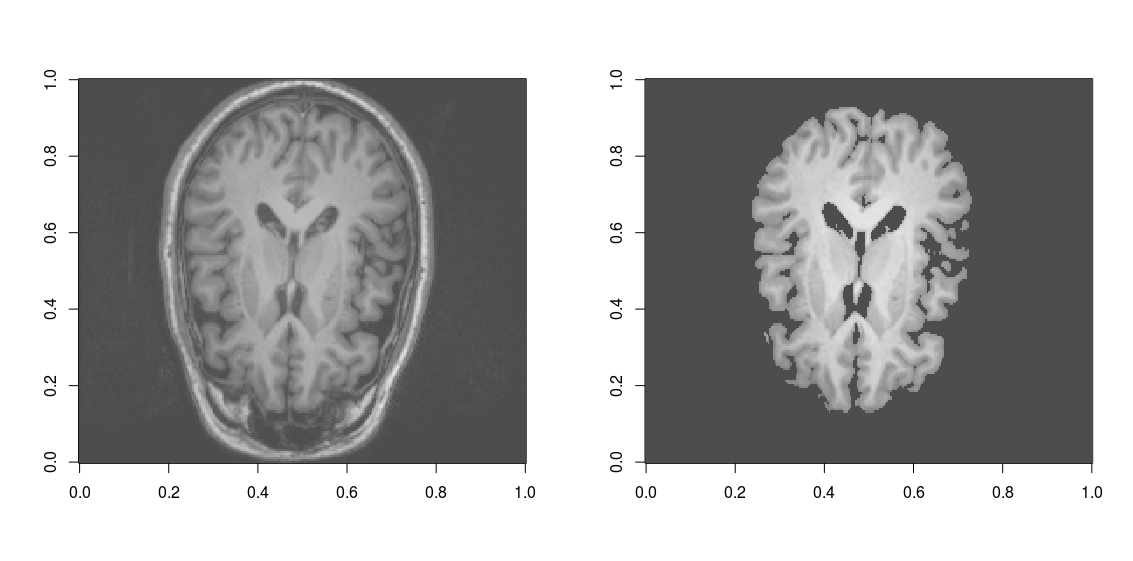
\includegraphics[width=\linewidth]{Images/6_t1_soft_eg.png}
\caption{Original T1-weighted image and the extracted soft tissue.}
\label{data-t1-soft-fig}
\end{figure}

\section{Generating response arrays}\label{data-lacune}

The T1-weighted and \textsc{flair} scans were rated visually by trained clinicians in accordance to the \textsc{strive} criterion \cite{WardlawJ.M.2013Nsfr}. The clinicians visually analysed the scans slice by slice, identifying possible lacunes, perivascular spaces, and other lesions. Each lesion was analysed by a team of clinicians to confirm the identification. The rating of lacunes was logged in Microsoft Excel, which details the scan ID and number of lacunes in each \textsc{mri} scan. For each lacune detected, the spreadsheet lists the axial slice ($y$ coordinate), diameter in millimetres, whether the lacune occurs on the left or right side of the brain, and the ID of the surrounding brain structure. Sample spreadsheet data is shown in Table \ref{data-excel-tab}.

\begin{table}[ht]
	\centering
	\begin{tabular}{llllll}
	\toprule[1.5pt]
	Scan ID & No. of lacunes & Axial Slice & Diameter & Side & Region\\
	\midrule
	42 & 2 & 102 & 7 & L & 3 (Cortex)\\
	102 & 1 & 112 & 10 & R & 4 (Thalamus)\\
	\ldots\\
	\bottomrule[1.5pt]\\
	\end{tabular}
	\caption{Sample spreadsheet data. Each row describes one scan, identifying the size and location of lacunes. Each row contains repeated columns to describe multiple lacunes per row.}
	\label{data-excel-tab}
\end{table}

The provided data describes the approximate anatomical location of lacunes. This format is not immediately usable to the model as it lacks precise coordinates. To resolve this, the spreadsheet was used as a guide to visually identify lacunes. Once found, an overlay of lacunes for the T1-weighted scans was generated such that each pixel in the image corresponds to a positive binary response value.

\begin{figure}[ht]
\centering
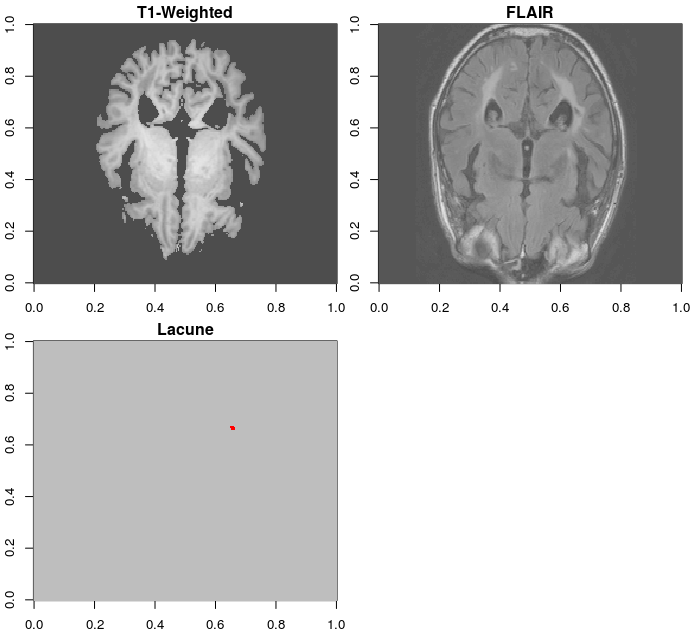
\includegraphics[width=\linewidth]{Images/6_lacune_mask.png}
\caption{Comparison of T1-weighted images, corresponding \textsc{flair} and lacune identification overlay (lacune in red).}
\label{data-t1-flair-lac}
\end{figure}

The responses were generated in FSLView, a program used by neuroscientists to view and annotate \textsc{mri} scans in the \texttt{.nifti} file format. For each brain scan described in the Excel spreadsheet, FSLView was used to generate a zero-initialised three-dimensional array of the same dimensions as the corresponding T1-weighted scan. Lacunes were visually identified by examining the indicated brain structure for lesions that appear dark in the T1-weighted images and with a hyperintense rim in the \textsc{flair} images. The empty arrays were opened in FSLView such that the voxels correspond to that of the T1-weighted images. The pixels that form the identified lacunes are filled with 1s using the Brush tool. These overlays are saved as \texttt{.nifti} files so they can be imported alongside the soft-tissue and \textsc{flair} \texttt{.nifti} files. An example of a lacune overlay is shown in Figure \ref{data-t1-flair-lac}.



% Start descriptions of data - where it came from. Rating process and wave reviews. Data itself consisted of t1 and flair scans, and excel spreadhseet of slice numbers and sizes. To build the response values, an overlay was made for each scan. Overlays were built in fslview in the nifti format. Lacunes were identified using the guidance spreadsheet. A brush tool was used to fill 1s for lacunes. 0 elsewhere.

\section{Generating samples}\label{data-samples}

The candidate generation model by Ghafoorian et al. \cite{GhafoorianM.2017Dml3} specifies each sample to be 51$\times$51 axial images of both T1-weighting and \textsc{flair}. In their model, samples were chosen randomly such that positive lacune samples encompassed one-third of the data set. Data augmentation was used to increase the number of samples. In total, Ghafoorian et al. collected $3.2\times10^5$ training samples from 1075 scans.

Our data set contains significantly fewer scans. In total the data set contains 411 \textsc{mri} scans, of which 35 contain lacunes. The scans were imported into R and converted into three-dimensional arrays using the AnalyzeFMRI package (v1.1-17). Each value of an array is the signal intensity of the scan at that voxel. Regions external to the scanned brain are given an intensity of 0.

The locations of the positive samples (lacunes) were extracted using the overlays generated in FSLView. Each nonzero value in the overlay was indexed and stored in a list. Two 51$\times$51-dimensional arrays were extracted from the T1-weighted and \textsc{flair} images such that the sample point occurs at the centre. To increase sample size, these images were augmented by flipping the image horizontally and adding them to the dataset. Examples are shown in Figure \ref{data-positives}. This method of sampling returned 3846 lacune samples in total.

\begin{figure}[ht]
\centering
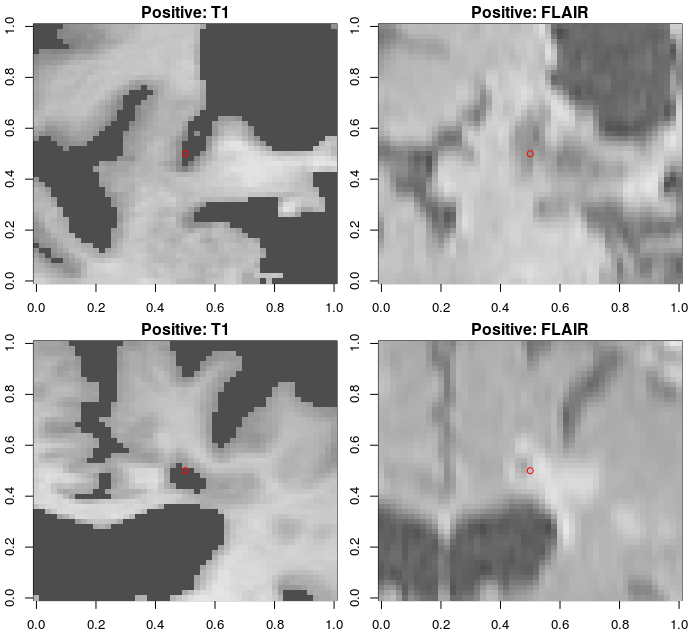
\includegraphics[width=\linewidth]{Images/6_positives.png}
\caption{Examples of positive samples. T1-weighted images and corresponding \textsc{flair}.}
\label{data-positives}
\end{figure}


\begin{figure}[ht]
\centering
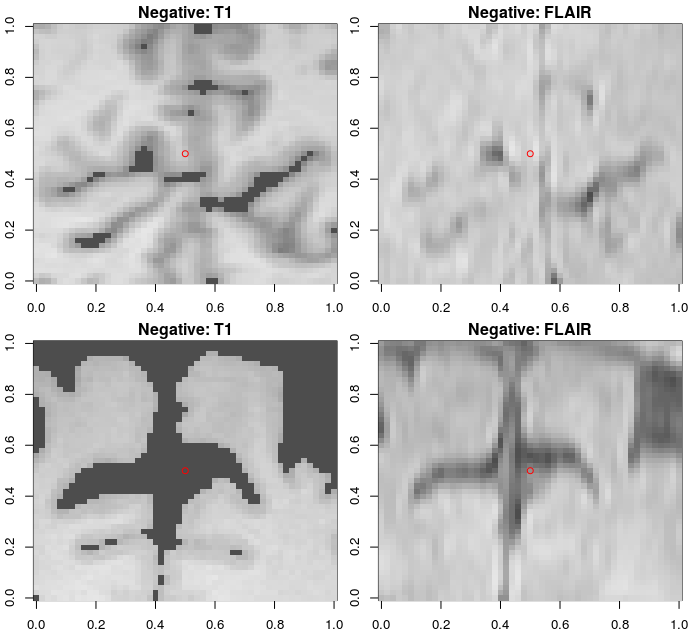
\includegraphics[width=\linewidth]{Images/6_negatives.png}
\caption{Examples of negative samples. T1-weighted images and corresponding \textsc{flair}.}
\label{data-negatives}
\end{figure}

Negative (non-lacune) samples were generated by sampling for points that returned 0 in the lacune overlay. Random samples were conducted by choosing sequential points as only around 10\% of the soft-tissue matrices are non-zero. A random starting pixel was chosen near the edge of the array. Further samples were 25 voxels apart in all three dimensions. Samples were discarded if they had a positive lacune response. Samples were also discarded if the centre 4$\times$4$\times$4 volume was entirely empty as the soft-tissue arrays are very sparse. Examples are shown in Figure \ref{data-negatives}. This was used to generate a total of 39983 negative samples. Positives samples make up 8.78\% of the dataset.

%\section{The Data}
%
%Where the data came from. The MRI source, type of images, with wavelengths etc. Similar description to Ghafoorian's (Section 2.1). Any preprocessing.
%
%What the samples were. E.g. 51x51 patches. Number of training, validation, testing.
%
%Show some example images, alongside their classification.
%
%The system that the models were built under - built in R using a tensorflow API. Models were run on dedicated servers.

%\section{First Model Structure}
%
%Code in Appendix.
%
%Purpose was to have a point of comparison against the model built by Ghafoorian et al. \cite{GhafoorianM.2017Dml3}.
%
%Brief outline of structure.
%
%Different number of samples. Far fewer lacunes in our dataset. Paper had 2/3 negatives, 1/3 positives. Our data consists of just under 10\% positives. Proposed model paper had 320K total samples. Our data has 50K, far fewer samples than the proposed model.
%
%In addition, around the 11th epoch, the training accuracy drops from near 100\% to near 0\%. This could be since the cross entropy has a log, and the algorithm attempts to take log(0). Introduce a small constant to achieve log(y + 1e-10).
%Getting NANs from the cross entropy function.
%
%
%\section{Proposed Model Structure}
%
%Code in Appendix.
%
%Explain structure of model, including diagram similar to that from Ghafoorian. Number of layers, number of neurons in each layer. What each layer was and the order. Method for chosen hyper-parameters. 


%%%%%%%%%%%%%%%%%%%%%%%%%%%%%%%%%%%%%%%%%%%%%%%%%%%%%%%%%%%%%%%%%%%%%%%%%%

\clearpage

\addcontentsline{toc}{chapter}{References}

\bibliographystyle{apalike}
\bibliography{bibliography.bib}

%\bibliographystyle{apacite}
%\bibliography{mybib.bib}

